\section{Results} \label{Results}

Figure \ref{ResultsPlot} shows estimated dynamic treatment effects and 95\% confidence intervals for all students and the four subgroups of interest. 

\begin{figure}[!h]
	\centering
	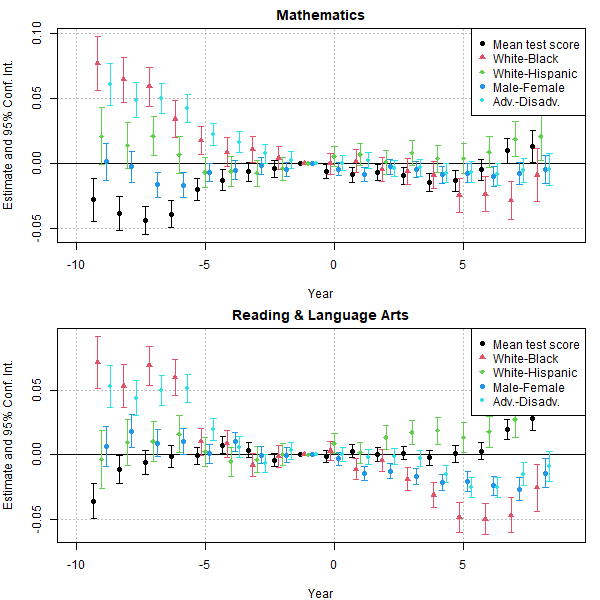
\includegraphics[scale=1]{"../Code & Data/ResultsPlot.pdf"}
	\caption{Dynamic Treatment effects in relative time: FEMA disaster data}
	\label{ResultsPlot}
\end{figure}


For the period of treatment there is a significant\footnote{Significant is used here in the sense that a confidence interval with nominal coverage of 95\% does not include zero, that is a corresponding t-test would reject the null hypothesis of a zero effect at the 5\% level.} effect of natural disasters on the performance in mathematics. The effect size is between just above zero and -0.01 standard deviations. For all subsequent periods the effect is not significant. There are some point estimates well below zero, but the uncertainty around those is relatively large. For performance in RLA, there are no significant effects.

Note that the number of observed units decreases with the distance in time from treatment. The reason for this is that in order to experience eight treated years, the county has to experience its first disaster very early. Similarly, it has to receive treatment very late to experience more than five years before treatment. As a result, the uncertainty increases with the distance in time from treatment.

For the subgroups we find some surprising results. Black students seem to perform better in RLA in the medium term after a disaster. That is, there are significantly positive results one to seven years after treatment. The effect sizes are substantial: Seven years after treatment the increase in RLA performance goes up to 0.1 standard deviations. In other words, the average black student sees an increase in performance of up to 0.1 standard deviations of the national reference cohort. Also, hispanic students score significantly lower in mathematics in the year following a disaster.



Positive effects of disasters on performance are not unheard of in the literature. In fact, this is somewhat consistent with the findings by \cite{Sacerdote_2012}. Many students have to switch schools and some may even benefit from attending a higher quality school after the disaster. Black students may disproportionally attend lower quality schools and are therefore more likely to benefit from having to switch schools. 

Figures \ref{ResultsPlotStorm} shows the same graphs based on the storm treatment. The results look very similar. In the period of the storm there is a significant decrease in mathematics scores of up to -0.015 standard deviations. For the years following treatment there are no significant effects.

For female students there is a significant decrease in both subjects in the period of the storm. For RLA we even find a significantly negative effect one year after the storm. Similarly, economically disadvantaged students perform worse in the period of treatment and in RLA one year after treatment. The effect sizes range from barely above zero up to -0.015 or even -0.02 standard deviations. For black and hispanic students we do not find any significant effects of the storm treatment.

\begin{figure}[!h]
	\centering
	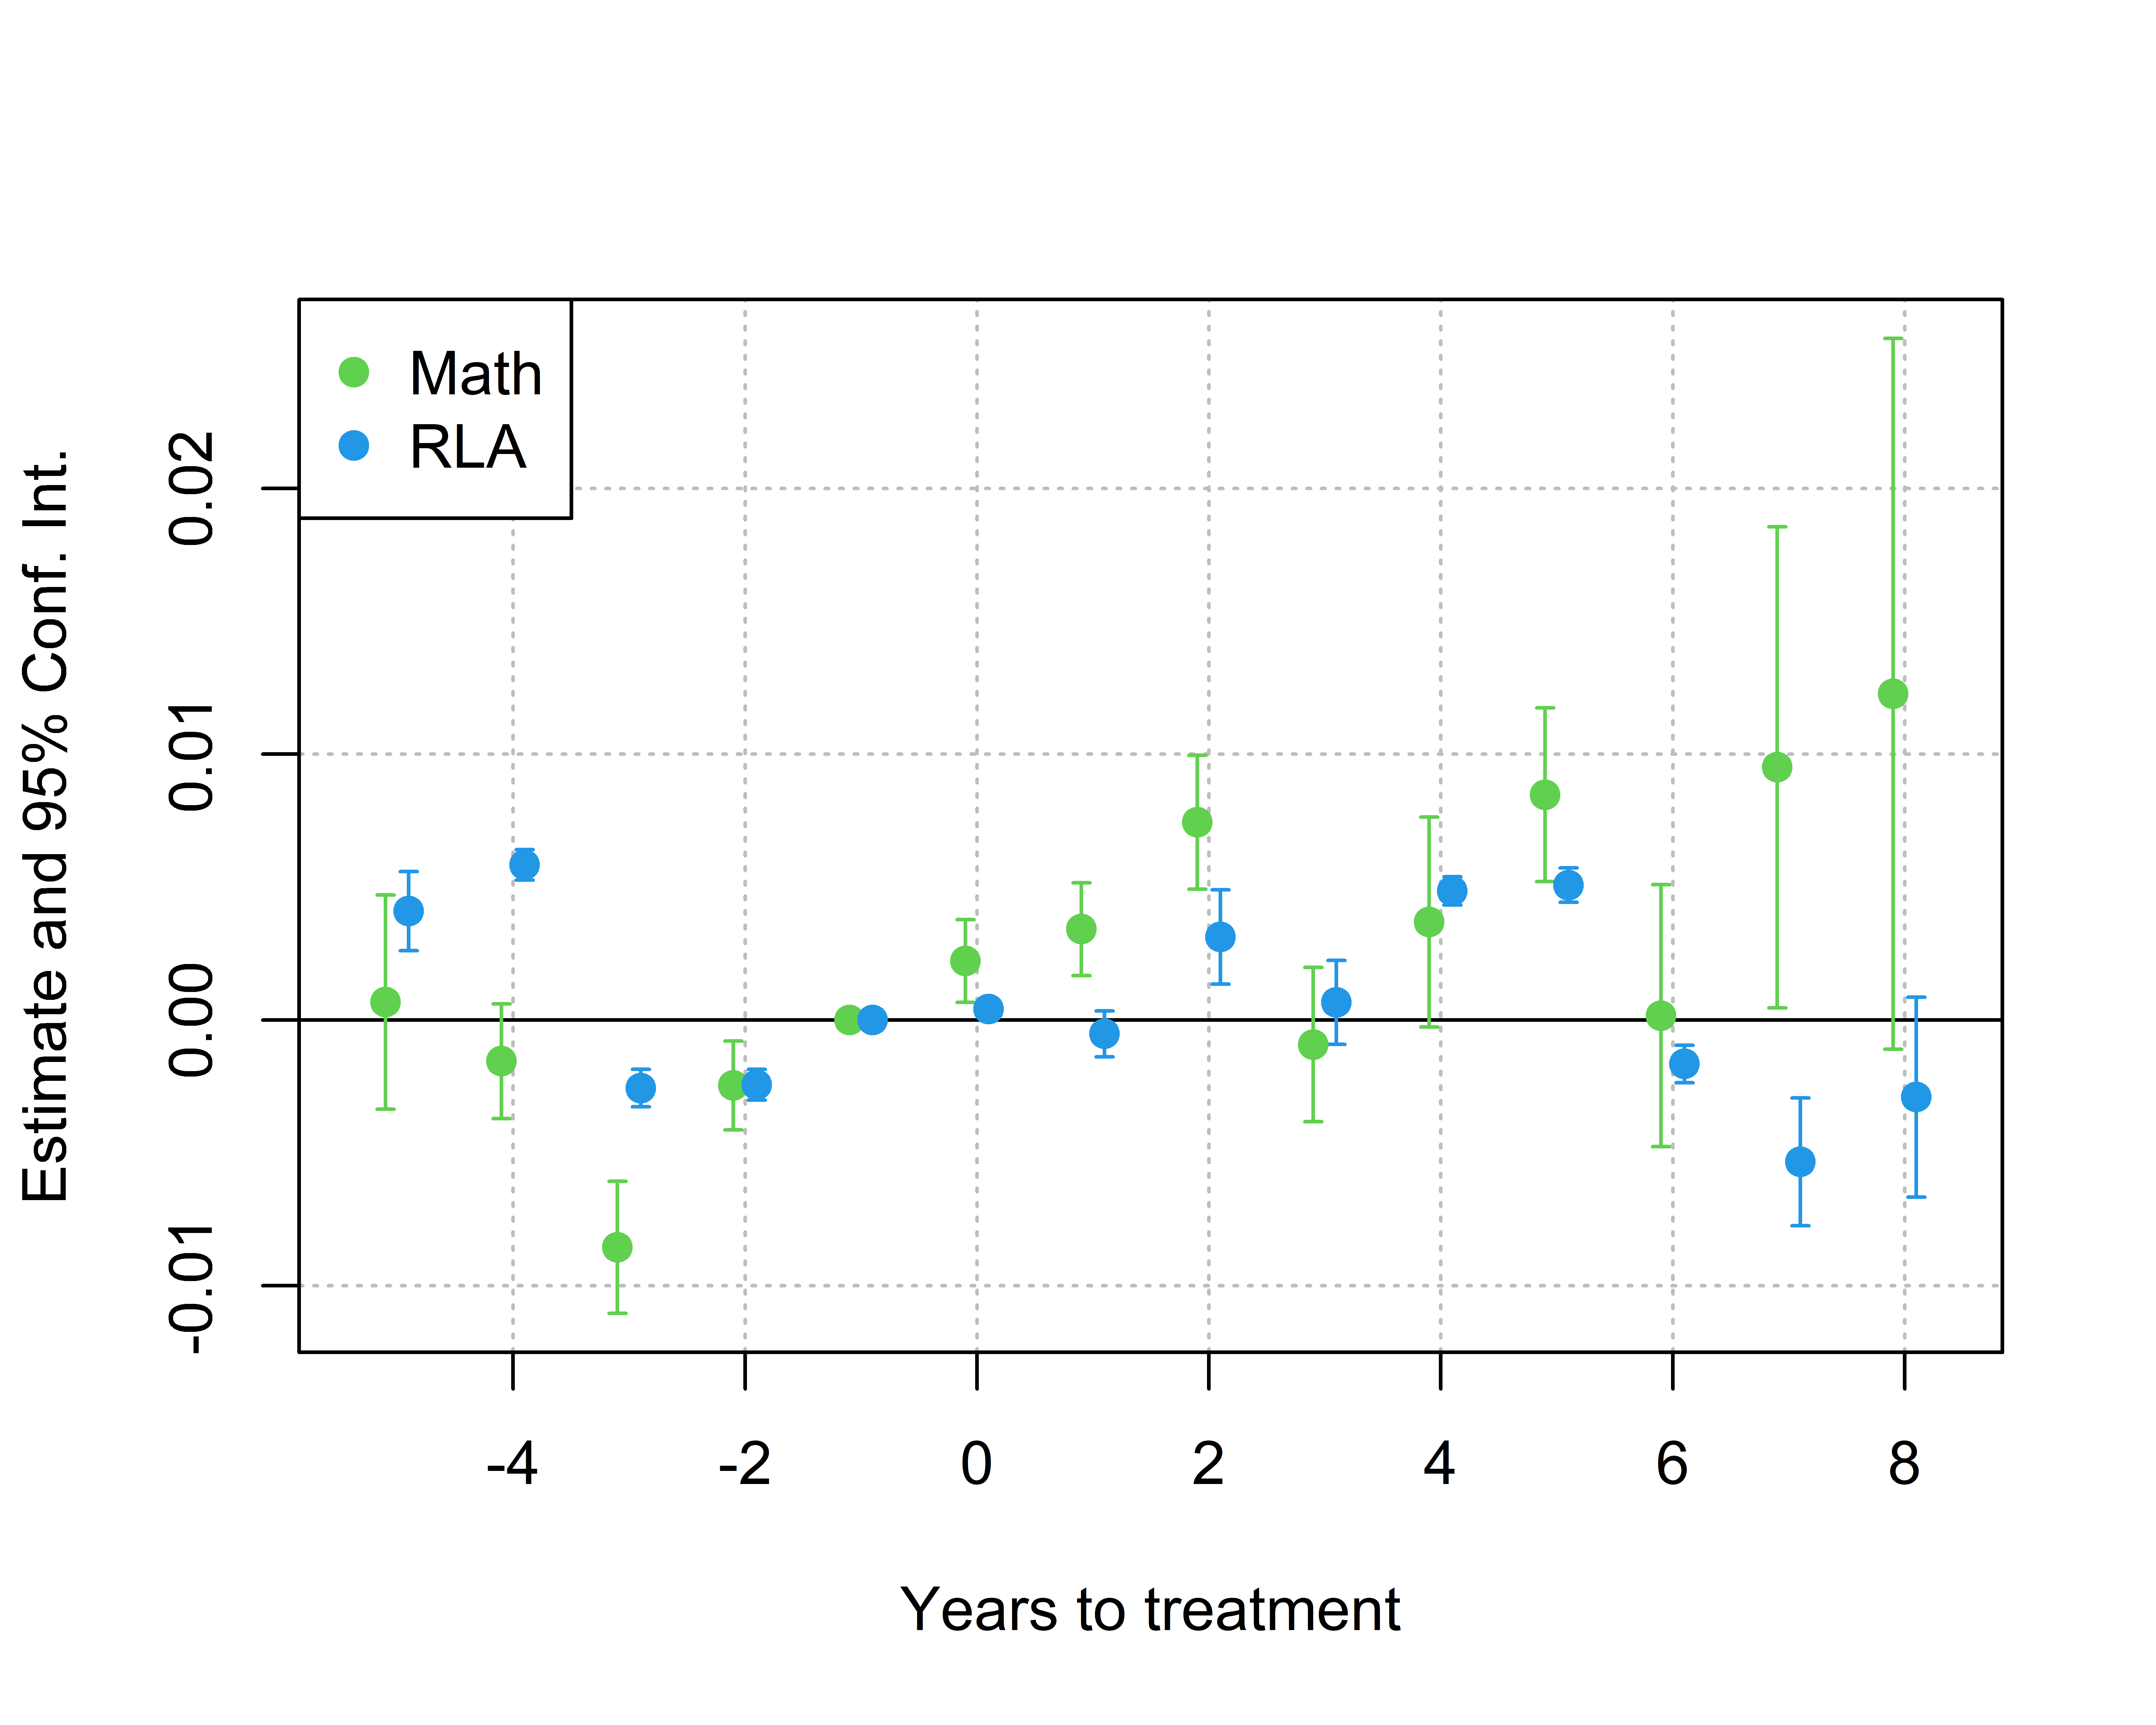
\includegraphics[scale=1]{"../Code & Data/ResultsPlotStorm.pdf"}
	\caption{Dynamic Treatment effects in relative time: NWS storm data}
	\label{ResultsPlotStorm}
\end{figure}


It could be the case that medium- and long-term effects are largely driven by migration. That's why it may be interesting to have a look at the ethnic composition of the counties relative to initial treatment. Figure \ref{EthnicComposition} shows ethnic shares for the treated counties in relative time.

\begin{figure}[!h]
	\centering
	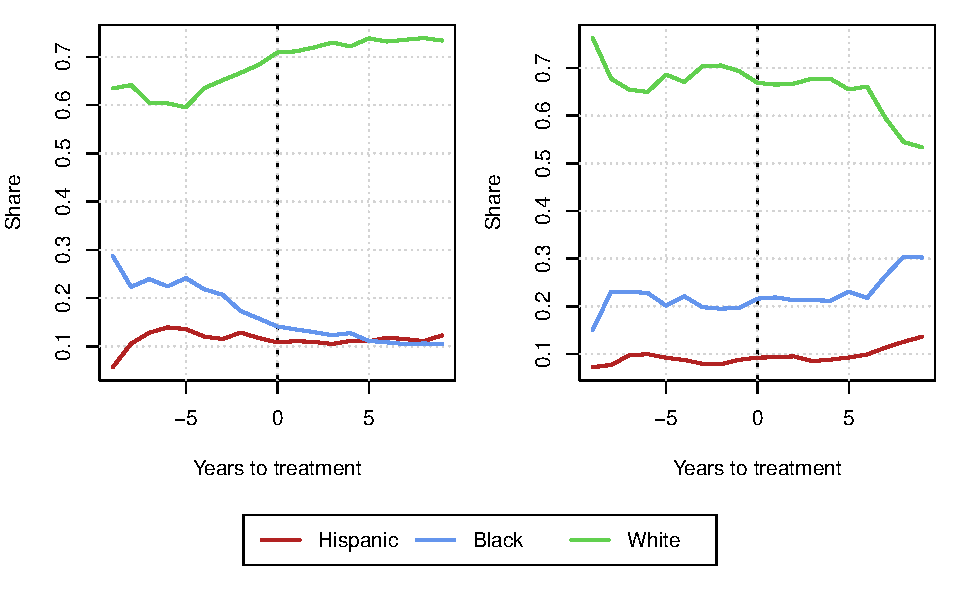
\includegraphics[scale=1]{"../Code & Data/EthnicComposition.pdf"}
	\caption{Aggregated ethnic shares by treatment timing based on FEMA disasters (left) and on NWS storms (right)}
	\label{EthnicComposition}
\end{figure}

In the left panel we see that the share of black students decreases in counties that experienced a disaster. This supports the hypothesis that black students disproportionately switch schools after disasters and may explain the positive long term effect as described above. However, the share of black students already decreases before treatment, so this may not be a causal effect of the disaster.

The same plot based on the NWS storm data shows a different picture. Here, all three shares remain somewhat constant until five years fter treatment. Then the share of black students increases, while the share of white students decreases. This suggests that the migration response to storms may be qualitatively different than the response to other forms of disasters. At least for the storms data this does not seem to be a major driver of the results.

A more in-depth analysis of migration responses to natural disasters and their role in academic achievement is unfortunately not possible with this data. Prior research based on individual level data indicates that it does play an important role \citep[for example][]{Sacerdote_2012}.









